% document setup
\documentclass[12pt,a4paper]{article}
\usepackage[utf8]{inputenc}
\usepackage[ngerman]{babel}

% maths
\usepackage{amsfonts}
\usepackage{amssymb}
\usepackage{amsmath}

% utility
\usepackage[dvipsnames]{xcolor}
\usepackage{float}
\usepackage[colorlinks=false,linkbordercolor=red,urlbordercolor=red]{hyperref}
\usepackage{caption}
\usepackage[shortlabels]{enumitem}
\usepackage{tikz}

% useful commands
\newcommand{\qed}{\null\nobreak\hfill\square}
\newcommand{\textqed}{\\$\qed$}

% title, author etc.
\title{Analysis I, Blatt 5}
\author{
    Gruppe 11\\
    Lorenz Bung (Matr.-Nr. 5113060)\\
    \href{mailto:lorenz.bung@students.uni-freiburg.de}{\texttt{lorenz.bung@students.uni-freiburg.de}}\\
    Charlotte Rothhaar (Matr.-Nr. 4315016)\\
    \href{mailto:charlotte.rothhaar97@gmail.com}{\texttt{charlotte.rothhaar97@gmail.com}}
}
\date{\today}

% begin document
\begin{document}

\maketitle


\section*{Aufgabe 17}

\begin{enumerate}[(a)]
    \item Nach dem Quotientenkriterium konvergiert $\sum\limits_{n=0}^{\infty} \frac{n^2}{2^n}$ absolut, wenn\\
    $\lim\limits_{n \to \infty} \left|\frac{a_{n+1}}{a_n}\right| < 1$.

    Wir erhalten
    \begin{align*}
    \lim\limits_{n \to \infty} \left|\frac{a_{n+1}}{a_n}\right|
    &= \lim\limits_{n \to \infty} \left|\frac{\frac{(n+1)^2}{2^{n+1}}}{\frac{n^2}{2^n}}\right|
    = \lim\limits_{n \to \infty} \left|\frac{(n+1)^2}{2^{n+1}} \cdot \frac{2^n}{n^2}\right|
    = \lim\limits_{n \to \infty} \left|\frac{(n+1)^2}{2n^2}\right|\\
    &\overset{n \geq 0}{=} \lim\limits_{n \to \infty} \frac{(n+1)^2}{2n^2}
    = \lim\limits_{n \to \infty} \frac{n^2 + 2n + 1}{2n^2}.
    \end{align*}
    Aus den Koeffizienten des höchsten Grades der Polynome im Bruch ergibt sich
    $$\lim\limits_{n \to \infty} \left|\frac{a_{n+1}}{a_n}\right| = \lim\limits_{n \to \infty} \frac{n^2 + 2n + 1}{2n^2} = \frac{1}{2} < 1.$$
    Damit konvergiert die Folge nach dem Quotientenkriterium absolut, und nach Lemma 3.12.12 ist jede absolut konvergente Reihe konvergent. \textqed

    \item Wir wenden das Leibnizkriterium für alternierend relle Reihen auf $\sum\limits_{n=0}^{\infty} (-1)^n \frac{1}{2n+1}$ an:

    \begin{itemize}
        \item Die Folge $\frac{1}{2n+1}$ ist eine Nullfolge, da sie Teilfolge der harmonischen Folge ist (welche bereits eine Nullfolge ist).\quad$\checkmark$
        \item Es bleibt zu zeigen, dass $a_n := \frac{1}{2n+1}$ monoton fallend ist:

        $$a_{n+1} \leq a_n \Rightarrow \frac{1}{2(n+1)+1} \leq \frac{1}{2n+1} \Rightarrow 2n+1 \leq 2n+3.\quad\checkmark$$

        Die Folge $a_n$ ist also monoton fallend.
    \end{itemize}

    Somit konvergiert die Reihe $\sum\limits_{n=0}^{\infty} (-1)^n \frac{1}{2n+1}$ nach dem Leibnizkriterium.

    Für die absolute Konvergenz verwenden wir das Minorantenkriterium:

    $$\left|a_n\right| = \left|\frac{1}{2n+1}\right| = \frac{1}{2n+1} \geq \frac{1}{2n} \geq \frac{1}{n}.$$

    $\sum\limits_{n=0}^{\infty} \frac{1}{n}$ ist jedoch die harmonische Reihe, welche divergiert.

    Somit konvergiert die Reihe $\sum\limits_{n=0}^{\infty} (-1)^n \frac{1}{2n+1}$ nicht absolut. \textqed

    \item Wir wenden das Quotientenkriterium auf die Reihe\\
    $\sum\limits_{n=0}^{\infty} \binom{2n}{n} \frac{1}{2^{3n-1}} = \sum\limits_{n=0}^{\infty} \frac{2n!}{n! \cdot n!} \cdot \frac{1}{2^{3n-1}}$ an:

    \begin{align*}
        \lim\limits_{n \to \infty} \left|\frac{a_{n+1}}{a_n}\right|
        &= \lim\limits_{n \to \infty} \left|\frac{\frac{2(n+1)!}{(n+1!(n+1))} \cdot \frac{1}{2^{3(n+1)-1}}}{\frac{2n!}{n!n!} \cdot \frac{1}{2^{3n-1}}}\right|\\
        &= \lim\limits_{n \to \infty} \left|\frac{2(n+1)!}{(n+1)!(n+1)} \cdot \frac{1}{2^{3(n+1)-1}} \cdot \frac{n!n! \cdot 2^{3n-1}}{2n!}\right|\\
        &= \lim\limits_{n \to \infty} \left|\frac{(2n+2) \cdot 2n!}{(n+1)n! \cdot (n+1)n! \cdot 2^{3n+2}} \cdot 2^{3n-1}\right|\\
        &= \lim\limits_{n \to \infty} \left|\frac{2(n+1) \cdot 2^{3n-1}}{(n+1)(n+1) \cdot 2^{3n} \cdot 2 \cdot 2}\right|\\
        &= \lim\limits_{n \to \infty} \left|\frac{2^{3n}}{(n+1) \cdot 2^{3n} \cdot 4}\right|
        = \lim\limits_{n \to \infty} \left|\frac{1}{4(n+1)}\right|\\
        &= \lim\limits_{n \to \infty} \left|\frac{1}{4} \cdot \frac{1}{n+1}\right|
        = 0 < 1.
    \end{align*}

    Damit konvergiert die Reihe $\sum\limits_{n=0}^{\infty} \binom{2n}{n} \frac{1}{2^{3n-1}}$ nach dem Quotientenkriterium absolut. \textqed
\end{enumerate}


\section*{Aufgabe 18}

\begin{enumerate}[(a)]
    \item Wir berechnen den Konvergenzradius $R$ der Potenzreihe $\sum\limits_{n=0}^{\infty} \frac{1}{n^n}x^n$ mithilfe von Satz 3.12.25.
    Damit ist
    \begin{align*}
        R &= \frac{1}{\limsup\limits_{n \to \infty} \sqrt[n]{|a_n|}}
        = \frac{1}{\limsup\limits_{n \to \infty} \sqrt[n]{\frac{1}{n^n}}}\\
        &= \frac{1}{\limsup\limits_{n \to \infty} \sqrt[n]{\left(\frac{1}{n}\right)^n}}
        = \frac{1}{\limsup\limits_{n \to \infty} \frac{1}{n}}\\
        &= \frac{1}{0} = \infty.
    \end{align*}

    \item Wir erhalten für die Potenzreihe $\sum\limits_{n=0}^{\infty} \frac{\sqrt{n2^n}}{(n+1)^4}x^n$ die Folge $a_n := \frac{\sqrt{n2^n}}{(n+1)^4}$ und somit
    \begin{align*}
        R &= \frac{1}{\limsup\limits_{n \to \infty} \sqrt[n]{|a_n|}}
        = \frac{1}{\limsup\limits_{n \to \infty} \sqrt[n]{\frac{\sqrt{n2^n}}{(n+1)^4}}}\\
        &= \frac{1}{\limsup\limits_{n \to \infty} \sqrt[n]{\sqrt{2^n} \cdot \frac{\sqrt{n}}{(n+1)^4}}}
        = \frac{1}{\limsup\limits_{n \to \infty} \sqrt[n]{\frac{\sqrt{n}}{(n+1)^4}} \cdot \sqrt{\sqrt[n]{2^n}}}\\
        &= \frac{1}{\limsup\limits_{n \to \infty} \sqrt[n]{\frac{\sqrt{n}}{(n+1)^4}} \cdot \sqrt{2}}
        = \frac{1}{\sqrt{2}}.
    \end{align*}

    \item Hier erhalten wir für die Potenzreihe $\sum\limits_{n=0}^{\infty} \frac{n!}{n^n}x^n$ die Folge $a_n := \frac{n!}{n^n}$.

    Weiterhin nutzen wir die Stirling-Formel zur Approximation von $n!$ für große $n$:
    \begin{equation}
        \label{eq1}
        n! \simeq n^ne^{-n}\sqrt{2 \pi n}
    \end{equation}

    Wir erhalten also

    \begin{align*}
        R &= \frac{1}{\limsup\limits_{n \to \infty} \sqrt[n]{|a_n|}}
        = \frac{1}{\limsup\limits_{n \to \infty} \sqrt[n]{\frac{n!}{n^n}}}
        = \frac{1}{\limsup\limits_{n \to \infty} \frac{\sqrt[n]{n!}}{n}}\\
        &\overset{\text{(\ref{eq1})}}{=} \frac{1}{\limsup\limits_{n \to \infty} \frac{\sqrt[n]{\left(\frac{n}{e}\right)^n\sqrt{2 \pi n}}}{n}}
        = \frac{1}{\limsup\limits_{n \to \infty} \frac{\frac{n}{e} \sqrt[n]{\sqrt{2 \pi n}}}{n}}\\
        &= \frac{1}{\limsup\limits_{n \to \infty} e \sqrt[2n]{2 \pi n}}
        = \frac{1}{\limsup\limits_{n \to \infty} e \sqrt[2n]{2\pi} \sqrt[2n]{n}}
        = \frac{1}{e}.
    \end{align*}
\end{enumerate}


\section*{Aufgabe 19}

\begin{enumerate}[(i)]
    \item $p(z) = \sum\limits_{i=0}^d a_iz^i,\ a_i \in \mathbb{C},\ a_0 \neq 0$\\

    \textbf{zu zeigen}: Für jedes $\lambda \in \mathbb{C}$ existiert ein (komplexes) Polynom $q$ mit Grad $d-1$, sodass $p(z) - p(\lambda) = (z - \lambda) q(z)$.\\

    \textbf{Beweis}:\\
    $p(z)$ hat die Form
    $$p(z) = a_d z^d + a_{d-1} z^{d-1} + \ldots + a_1 z + a_0.$$
    Wir suchen
    $$q(z) = b_{d-1} z^{d-1} + b_{d-2} z^{d-2} + \ldots + b_1 z + b_0$$
    mit $q(z) = \frac{p(z)}{z - \lambda} - \frac{p(\lambda)}{z - \lambda}$.\\

    Durch Polynomdivision ergibt sich
    \begin{align*}
        q(z) = &(a_d z^d + a_{d-1} z^{d-1} + \ldots + a_1 z + a_0) : (z - \lambda) = a_d z^{d-1} + \ldots\\
        &\frac{-(a_d z^d - \lambda a_{d-1} z^{d-1})}{\vdots}
    \end{align*}

    Somit ist der Grad des entstehenden Polynoms $d-1$.
    Dies gilt ebenfalls für $p(\lambda)$.
    Auch bei Subtraktion entsteht ein Polynom vom Grad $d-1$.
    Somit existiert immer ein solches Polynom $q$.

    \item \textbf{zu zeigen}: Ist das Polynom $p(z) = a_d z^d + a_{d-1} z^{d-1} + \ldots + a_1 z + a_0$ vom Grad $d$, so hat $p(z)$ höchstens $d$ Nullstellen.\\

    \textbf{Beweis}:\\
    Sei $\lambda_1$ eine Nullstelle des Polynoms $p(z)$.
    Der Linearfaktor $(z - \lambda_1)$ lässt sich von $p(z)$ abspalten und wir erhalten
    $$p(z) = (z - \lambda_1) (a_{d-1} z^{d-1} + a_{d-2} z^{d-2} + \ldots + a_1 z + a_0),$$
    also nach Teilaufgabe (i) ein Restpolynom vom Grad $d-1$.
    Es lässt sich vom Polynom $p(z)$ also höchstens $d$-mal ein Linearfaktor abspalten.\\
    Jede Nullstelle wird durch mindestens einen der so entstandenen Linearfaktoren repräsentiert.
    Daher kann ein Polynom vom Grad $d$ also maximal auch $d$ Nullstellen besitzen.

    \item Aus dem in \autoref{fig:a19iii1} dargestellten Schema lässt sich erkennen:
    \begin{itemize}
        \item $a_d$ wird $d$-mal mit $x_0$ multipliziert, also $a_d {x_0}^d$
        \item $a_{d-1}$ wird $d-1$-mal mit $x_0$ multipliziert, also $a_{d-1} {x_0}^{d-1}$
        \item $\vdots$
        \item $a_0$ wird 0-mal mit $x_0$ multipliziert, also $a_0 x^0 = a_0$.
    \end{itemize}

    \begin{minipage}{\linewidth}
        \centering
        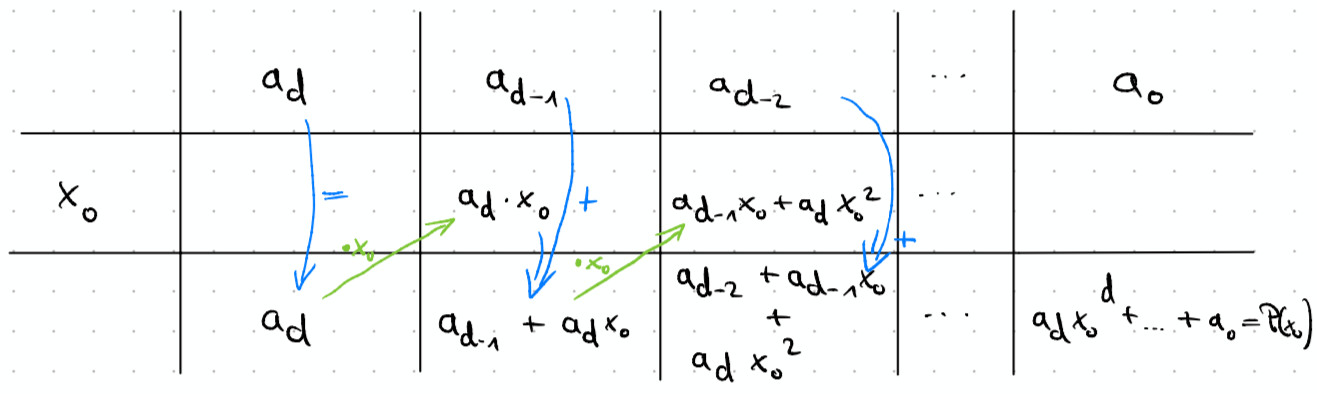
\includegraphics[width=0.75\textwidth]{a19iii1.jpg}
        \captionof{figure}{}
        \label{fig:a19iii1}
    \end{minipage}
    Es ergibt sich $a_d {x_0}^d + a_{d-1} {x_0}^{d-1} + \ldots + a_1x_0 + a_0 = p(x_0)$.
    Somit ist $p(x_0) = z$.

    \begin{minipage}{\linewidth}
        \centering
        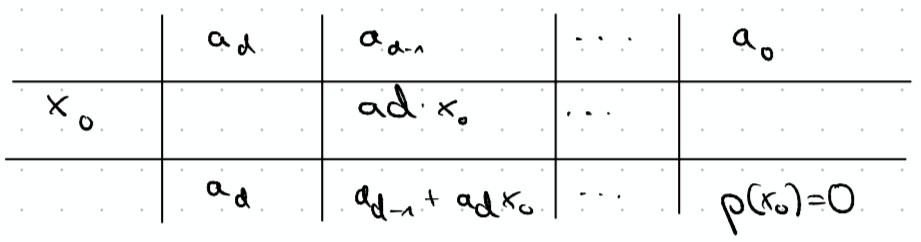
\includegraphics[width=0.75\textwidth]{a19iii2.jpg}
        \captionof{figure}{}
        \label{fig:a19iii2}
    \end{minipage}

    Wenn $x_0$ eine Nullstelle des Polynoms ist, erhalten wir nach dem in \autoref{fig:a19iii2} dargestellten Schema
    $$q(x) = a_d x^d + a_{d-1} x^{d-1} + \ldots + p(x_0).$$
    Damit ist
    $$q(x) \cdot (x - x_0) = a_d x^d + a_{d-1} x^{d-1} + \ldots = p(x).$$
\end{enumerate}


\section*{Aufgabe 20}

\begin{enumerate}[(i)]
    \item \textbf{Behauptung}: $(s_k)_{k>0}$ muss eine Nullfolge sein, damit $\sigma_n$ konvergiert.\\

    \textbf{Beweis}:
    Wie wissen: $\forall \varepsilon > 0 \exists N \in \mathbb{N}: |a_n| < \varepsilon\ \forall n \geq N.$\\
    Wir zeigen: $\forall \varepsilon > 0 \exists M \in \mathbb{N}: \left|\frac{s_1 + s_2 + \ldots + s_m}{m}\right| < \varepsilon\ \forall m \geq M.$

    Nach der Dreiecksungleichung gilt für $m > N$:
    $$\left|\frac{s_1 + s_2 + \ldots + s_m}{m} - 0\right| \leq \left|\frac{s_1 + s_2 + \ldots + s_N}{m}\right| + \left|\frac{s_{N+1} + s_{N+2} + \ldots + s_m}{m}\right|$$
    Sei $\varepsilon > 0$ vorgegeben.\\
    Da $\lim\limits_{n \to \infty} \sigma_n = 0$, ist $\forall \frac{\varepsilon}{2} \exists N \in \mathbb{N}: |\sigma_n - 0| = |\sigma_n| < \frac{\varepsilon}{2}\ \forall n \geq N.$\\
    Wir wählen $M > N$ und $\left|\frac{s_1 + \ldots + s_N}{M}\right| < \frac{\varepsilon}{2}.$
    Sei nun $m \geq M$. Dann ist

    \begin{align*}
        \left|\frac{s_1 + \ldots + s_m}{m}\right| &= \left|\frac{s_1 + \ldots + s_N + s_{N+1} + \ldots + s_m}{m}\right|\\
        &\overset{\Delta\text{-Ugl.}}{\leq} \frac{|s_1 + \ldots + s_N|}{m} + \frac{|s_{N+1}| + \ldots + |s_m|}{m}\\
        &< \frac{\varepsilon}{2} + \frac{|s_{N+1}| + \ldots + |s_m|}{m}
        \leq \frac{\varepsilon}{2} + \frac{(m-N)\frac{\varepsilon}{2}}{m}
        \leq \varepsilon.
    \end{align*}

    \item

    \item \pagebreak Ist $s_n := \sum\limits_{k=1}^\infty (-1)^{k+1}$ Cesaro-summierbar?\\
    Partialsummen:
    \begin{align*}
        s_1 &= 1\\
        s_2 &= 1-1 = 0\\
        s_3 &= 1-1+1 = 1\\
        &\ \vdots\\
        s_{2n} &= \sum\limits_{k=1}^{2n} (-1)^{k+1} = 0\\
        s_{2n+1} &= \sum\limits_{k=1}^{2n+1} (-1)^{k+1} = 1.
    \end{align*}
    Wir bilden $\sigma_n := \frac{1}{n} (s_1 + s_2 + \ldots + s_n)$:
    \begin{align*}
        \sigma_1 &= 1\\
        \sigma_2 &= \frac{1-0}{2} = \frac{1}{2}\\
        \sigma_3 &= \frac{1+0+1}{3} = \frac{2}{3}\\
        &\ \vdots\\
        \sigma_{2n} &= \sum\limits_{k=1}^{2n} s_k = \frac{n}{2n} \overset{n \to \infty}{\longrightarrow} \frac{1}{2}\\
        \sigma_{2n+1} &= \sum\limits_{k=1}^{2n+1} s_k
        = \frac{n+1}{2n+2}
        = \frac{2n+2}{2(2n+2)}
        = \frac{2n+1}{2(2n+2)} + \frac{1}{2(2n+2)}\\
        &= \frac{1}{2} + \frac{1}{2(2n+2)}
        \overset{n \to \infty}{\longrightarrow} \frac{1}{2} + 0
        = \frac{1}{2}.
    \end{align*}
    Also $\sigma_n \overset{n \to \infty}{\longrightarrow} \frac{1}{2}$ und damit ist der Cesaro-Grenzwert $\frac{1}{2}$.
\end{enumerate}


% end document
\end{document}